\documentclass[12pt]{scrartcl} %for better layouts
\usepackage{graphicx}
\usepackage{amsmath}
\usepackage{syntonly}
%\syntaxonly for quickly checking document


\title{The Effect of Oil Price on Field Production: Not Much}
\subtitle{Evidence from the Norwegian Continental Shelf}
\author{
  		Johannes Mauritzen \\
        Department of Business and Management Science\\
        NHH Norwegian School of Economics\\
        Bergen, Norway \\	           
		}
\date{\today}

\begin{document}
\maketitle

\begin{abstract}
This is the paper's abstract \ldots
\end{abstract}

\section{Introduction}

For most of the last century, crude oil has been the single most important and valuable fuel source in the world economy.  Naturally, questions of how the oil price affects the world economy as well as how oil production reacts to the oil price have been fundamental topics in economics. However a significant omission exists in the literature.  While several studies have taken up the issue of how oil prices affects searching for new fields, to my knowledge no field-level studies exist of the effects of oil prices on oil production at existing fields.  

The effect of oil prices on existing field level production is an important topic, both as an empirical counterpart to the extensive theoretical literature on optimal extraction and more generally in understanding the mechanisms of how total oil supply reacts in response to price.  

The lack of research on the role of price in oil field production is likely due to two main factors - the availability of data and the non-linear time profile of field production.  Most oil production has historically either been done by large private oil companies, notably “super majors” and more recently has been dominated by state-owned oil companies and national monopolies.  Both of these types of entities tend to consider field-level data as either company or state secrets.   

Luckily a notable exception to the general rule of inaccessible data exists.  The Norwegian government has committed itself to transparency in the petroleum sector and detailed data sets on most aspects of the country’s oil industry is openly available.  I use historical production data from all 77 currently or formerly oil-producing fields on the Norwegian continental shelf in order to estimate the effect that prices have on oil production.  

By looking only at the effect of price on fields that currently or previously have produced oil I am limiting the scope of this article.  The effect of oil prices on total production over an extended period of time is likely due to not just reactions in production in existing fields but also increased searching for new fields.  In fact, an implication of this work is that much of the total production response from higher oil prices is from increased searching.

The main finding in this article is that oil production at the field level has no significant reaction to concurrent changes in the oil price, where concurrent is broadly defined as within the first three years.  A slight effect can be detected at a lag of between 4 and 6 years, with a magnitude of about a 2 to 4\% increase in yearly production for a 10 dollar increase in the price of oil.  This effect is somewhat greater and with less of a lag in large fields compared to small fields.

The main methodological problem, as mentioned, is the non-linear production profile of oil fields.  Once full scale extraction is started in an oil field, pressure in wells will quickly drop.  Technological solutions such as gas and water injection also have quickly declining effectiveness.  In turn production will drop quickly.  The norwegian petroleum directorate estimates that only x percent of oil in most fields are recoverable. 

Oil field production is correlated across fields - that is, increases and decreases in production in fields are not randomly distributed across time.  Instead, as Figure 1 shows with the 10 largest Norwegian oil fields, production profiles tend to be correlated with each other.  The result is a total production curve that is bell shaped over time as figure 2 shows.  However since oil prices are autocorrelated, a failure to properly account for the production profile will lead to spurious estimation of the price terms in a regression.  

The direction of this bias can be gleaned in figure 2.  High oil prices were present at periods of relatively low production in the late 1970s and early 1980´s as well as the last 10 years, however real prices reached some of their lowest levels at the same time as the top of production around the year 2000.  This inverse relationship is of course entirely accidental, but will heavily bias the estimation of the effect of price on production if the production profile at the level of the oil field is not properly accounted for.  

\begin{figure}
	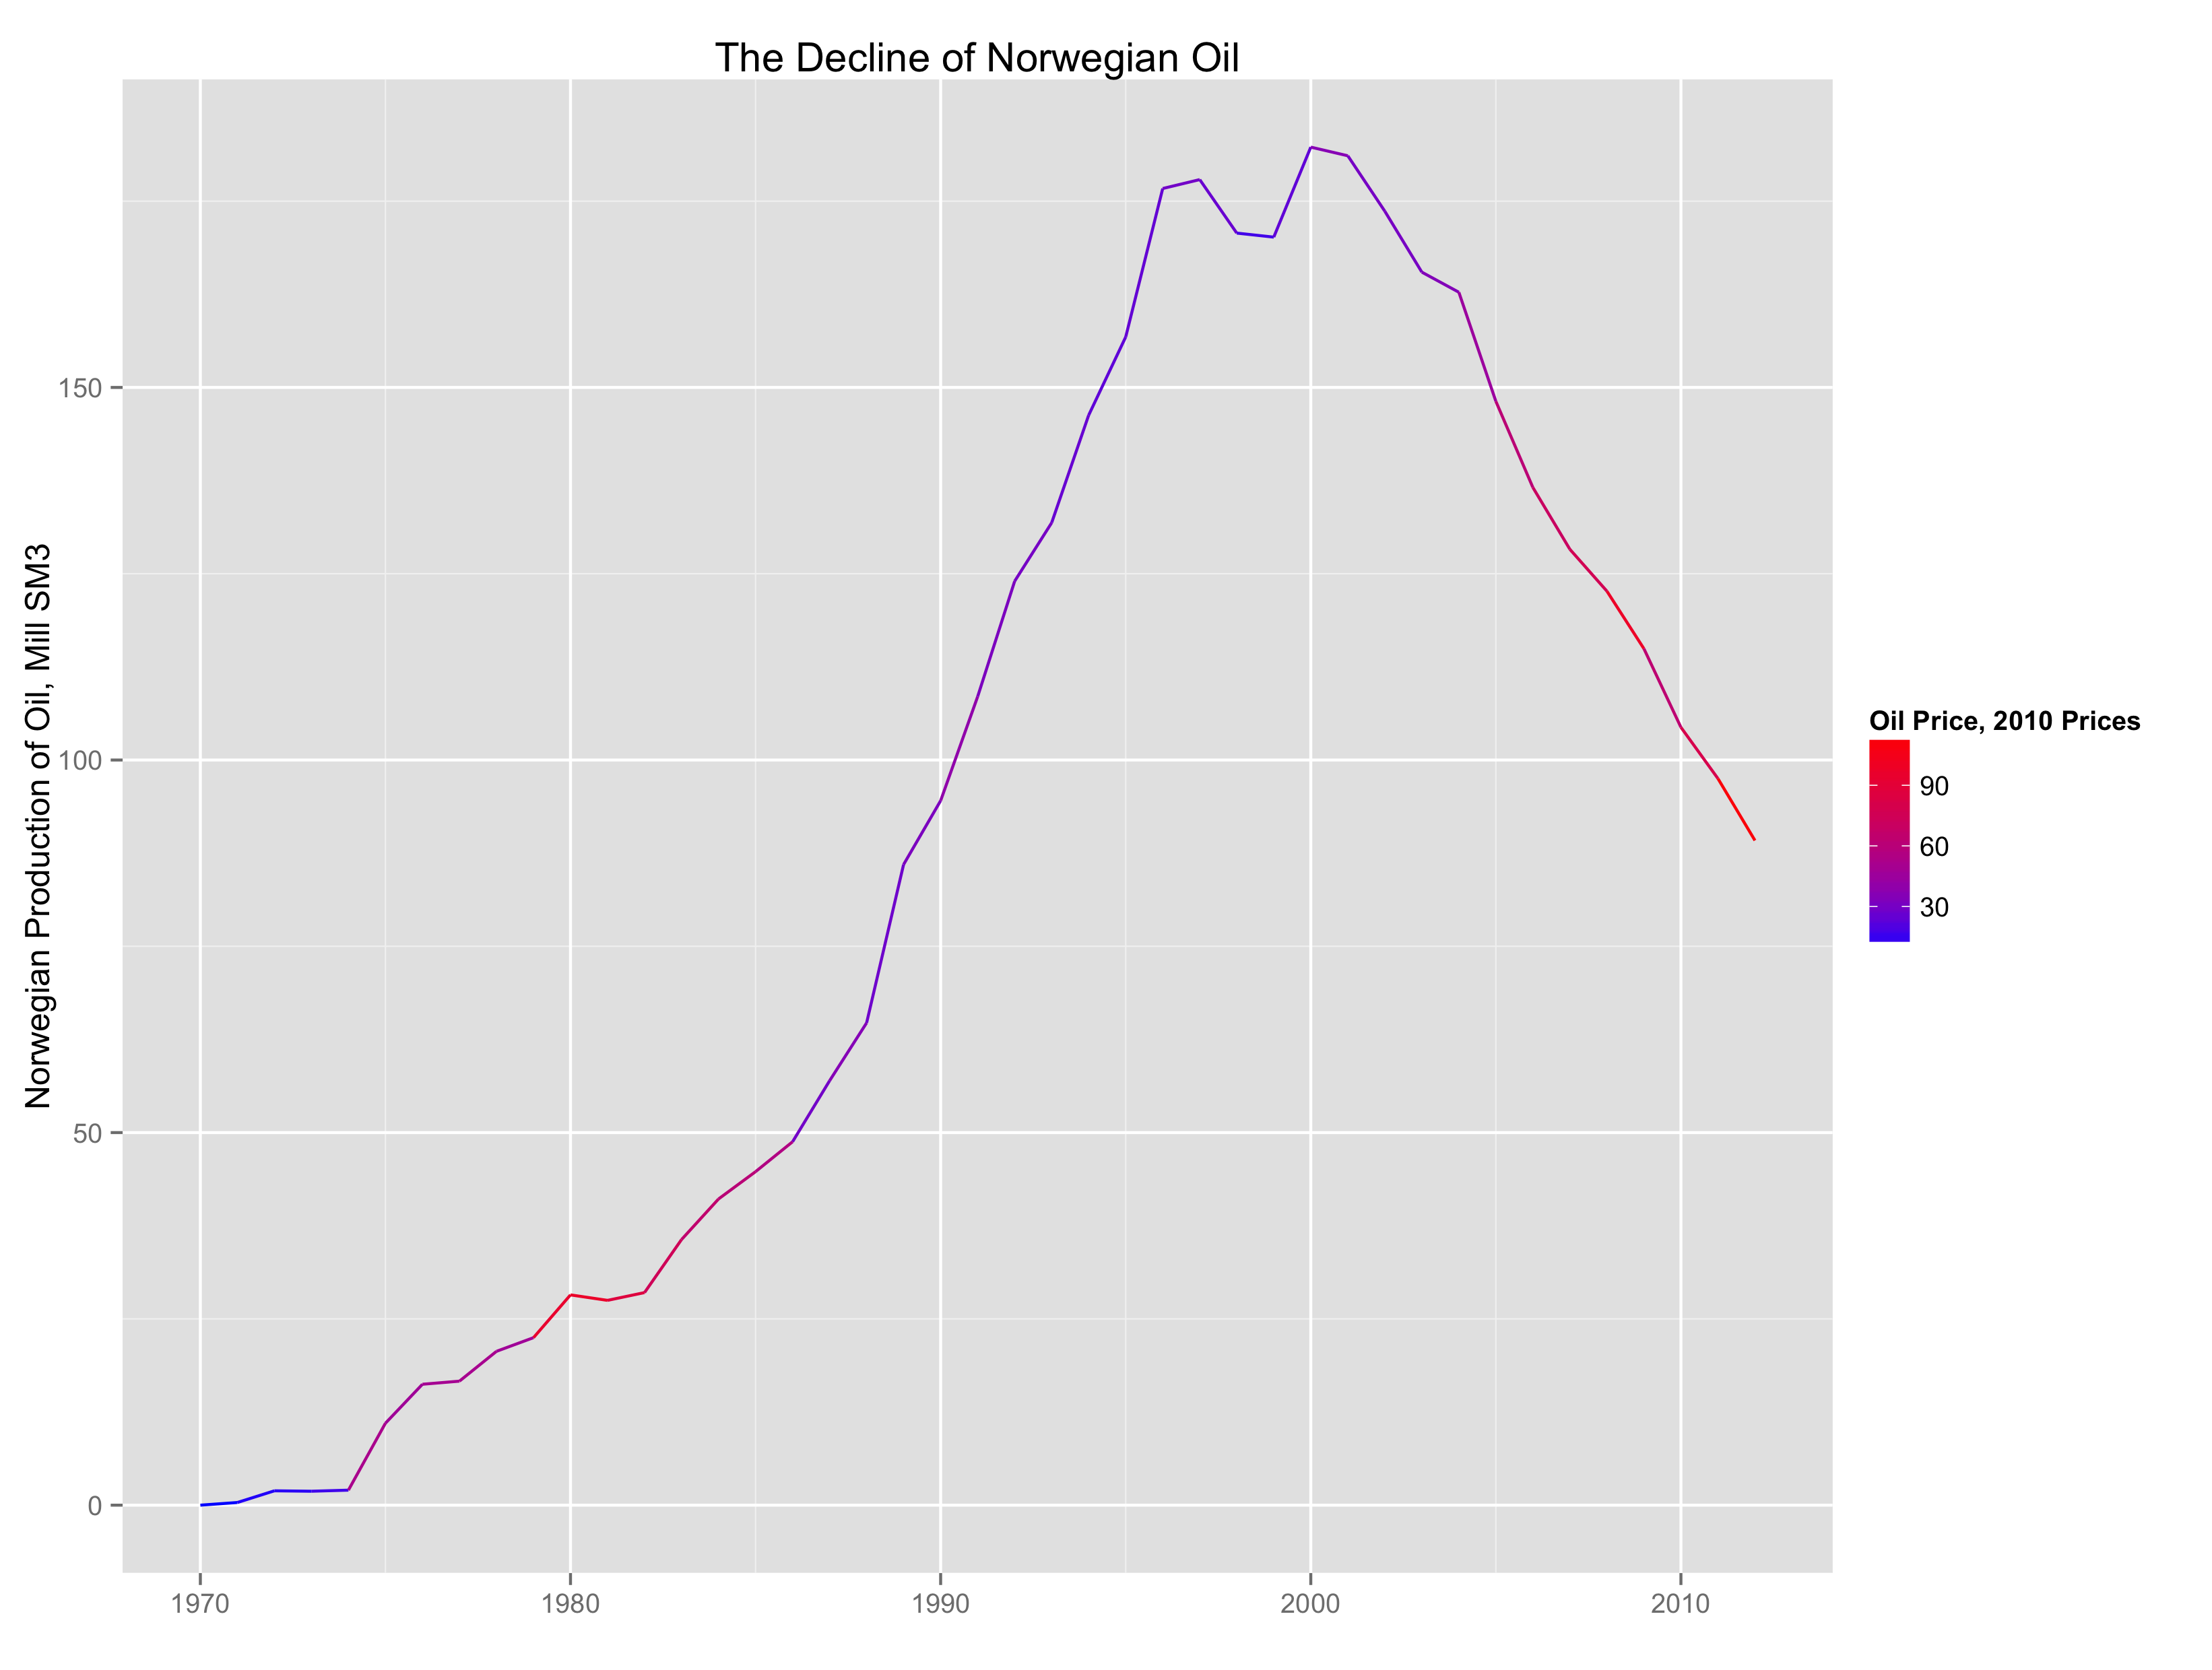
\includegraphics[width=1\textwidth]{oil_decline.png}
\end{figure}

\begin{figure}
	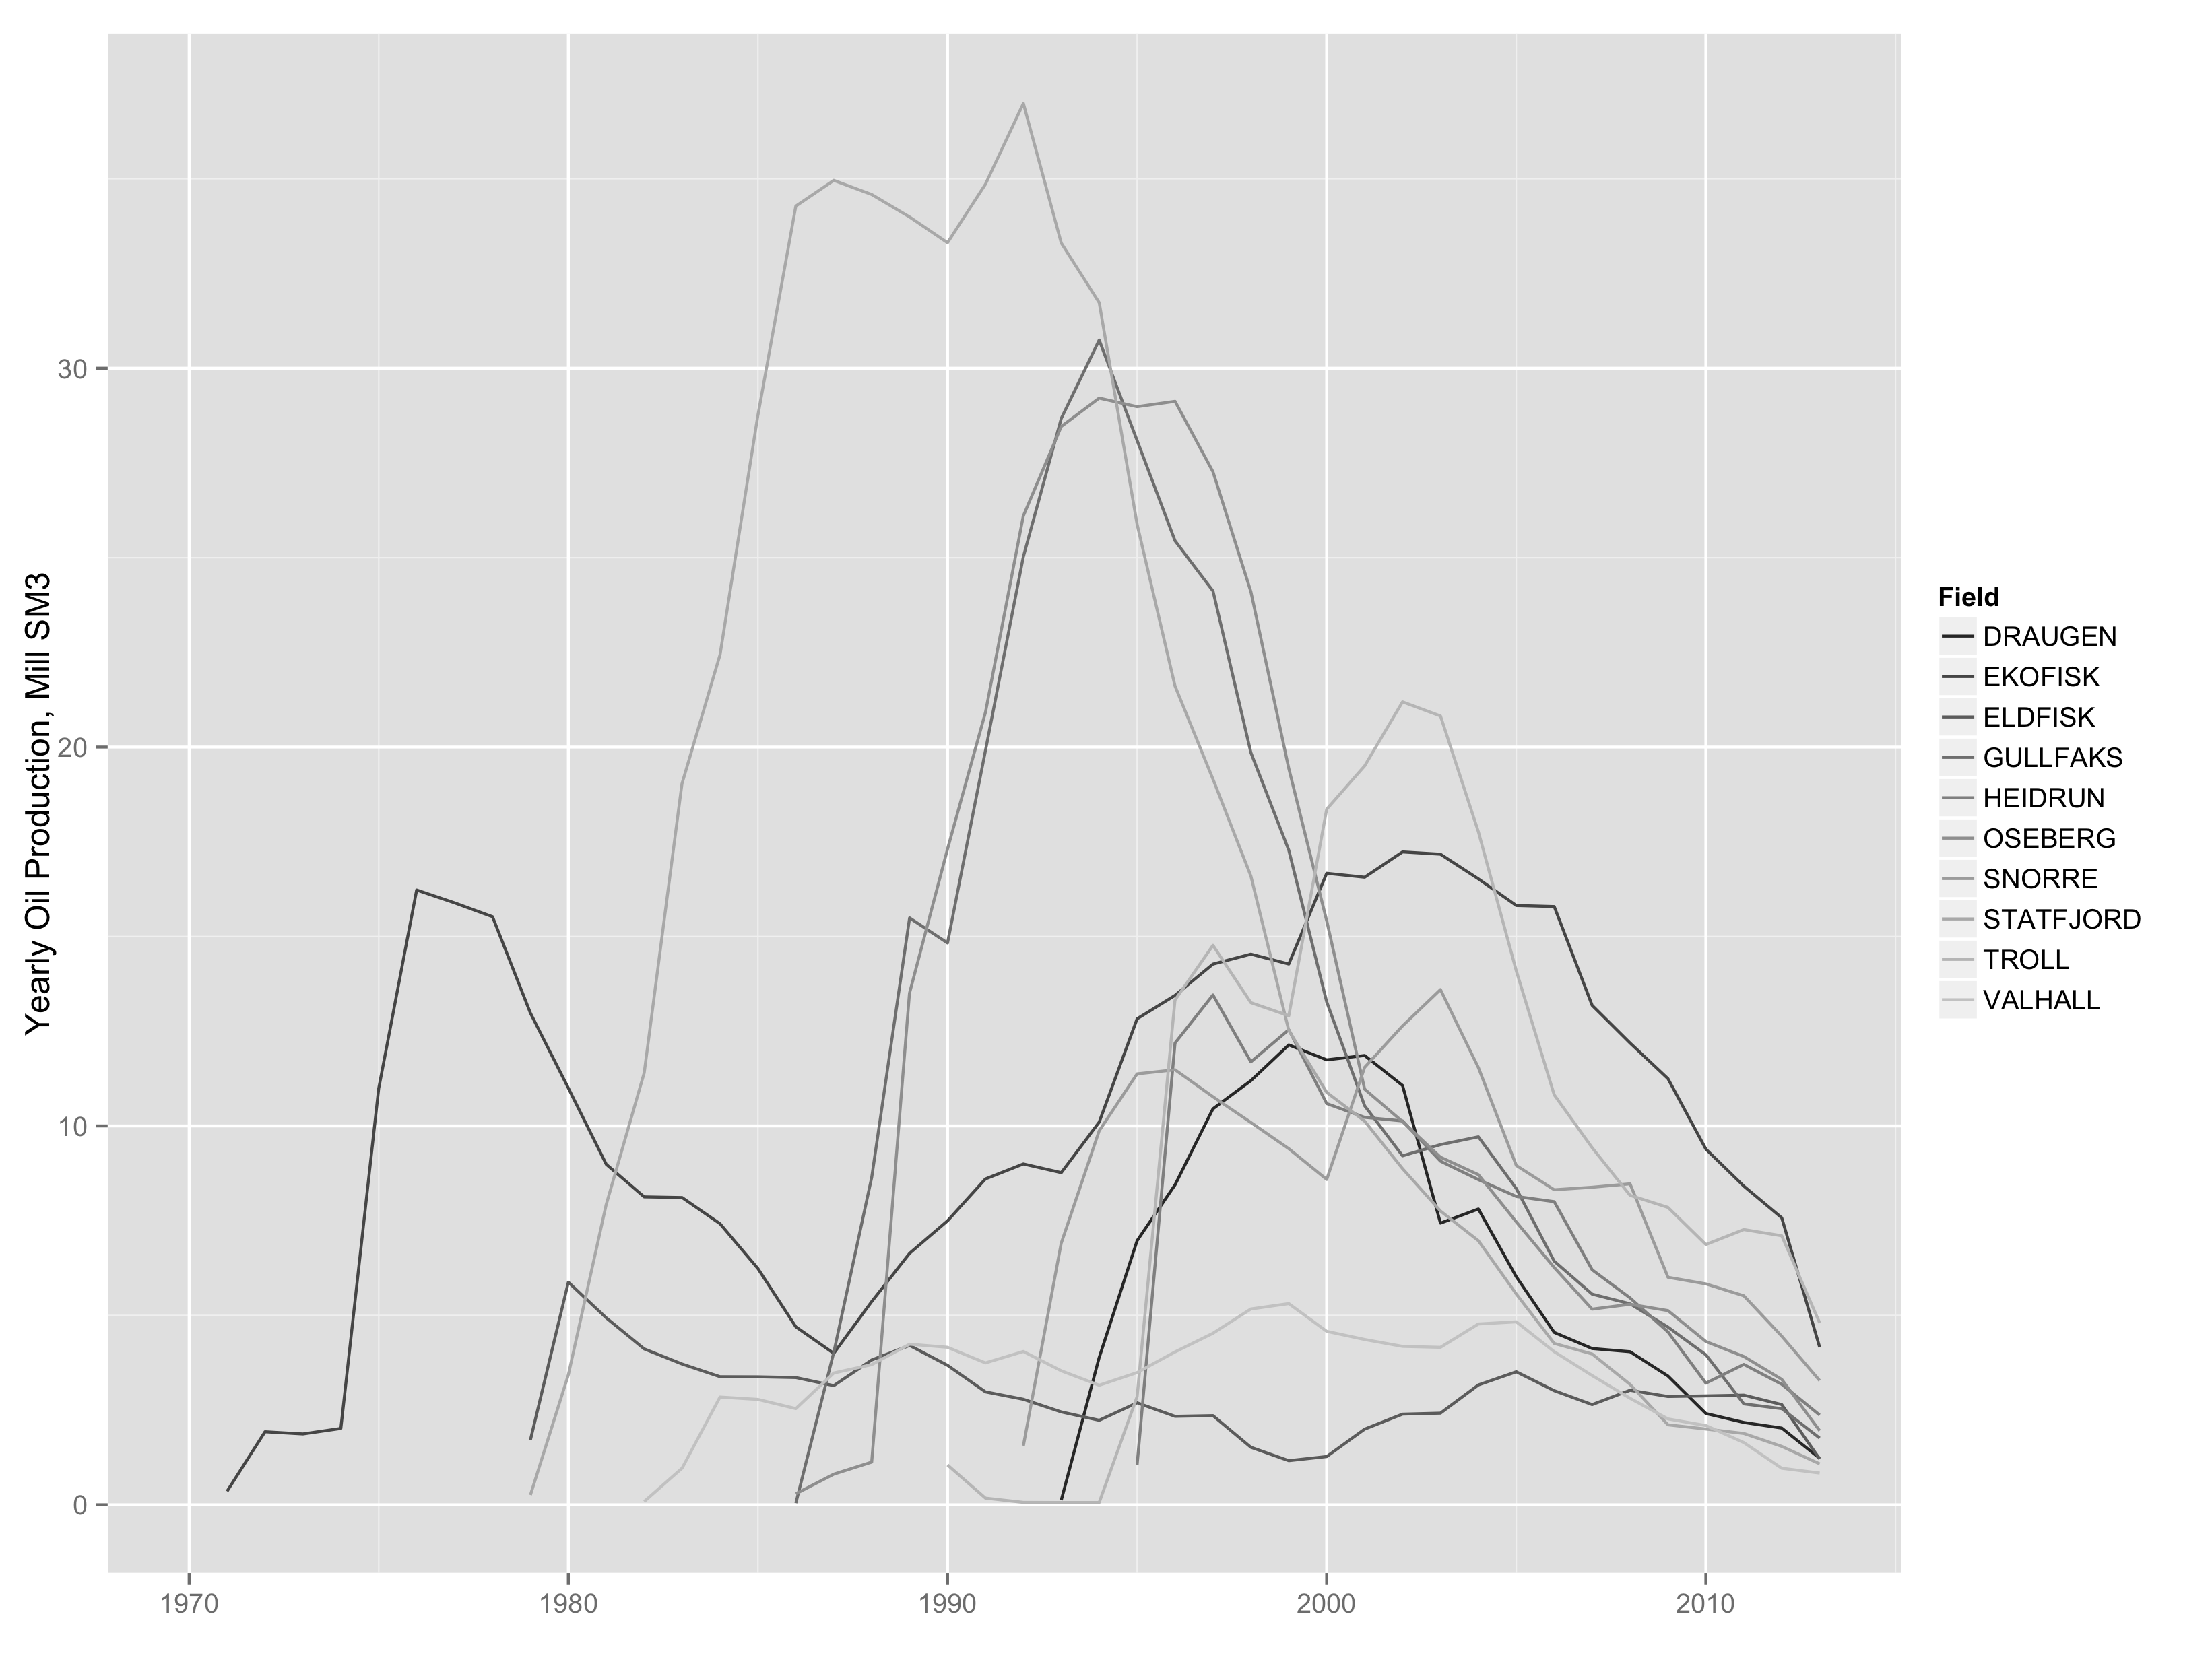
\includegraphics[width=.8\textwidth]{top10_production.png}
	\end{figure}

As a solution I use a semi-parametric model within the Generalized Additive Model frameworks of Tsibriani and X (cite).  Here I use a two-dimensional smoothed spline function to account for the general non-parametric shape of the production profile while price terms are represented linearly.  The coefficient on the price variable can then be seen as the average price effect.  

\section{The effect of oil price on production: theory and empirics}
The question of the effect of oil prices on production and the more general question of optimal oil extraction has a long history and goes back to the seminar work of hotelling31.  o

\section{Oil production on the Norwegian continental shelf}
The first commercial oil well in Norwegian continental waters was discovered in december of 1969 in what became the Ekofisk oil field, the largest Norwegian oil field by estimated recoverable reserves.  As figure 3 shows, most of the largest fields in the North Sea were found relatively early on while more recent finds have tended to be smaller.  A major exception to this trend was the recent find of the Johan Sverdrup field which is estimated to have approximately 300 million SM3 of recoverable oil.\footnote{The Johan Sverdrup field is estimated to begin producing oil in 2017 and so is not present in data set used for the analysis.}  

\begin{figure}
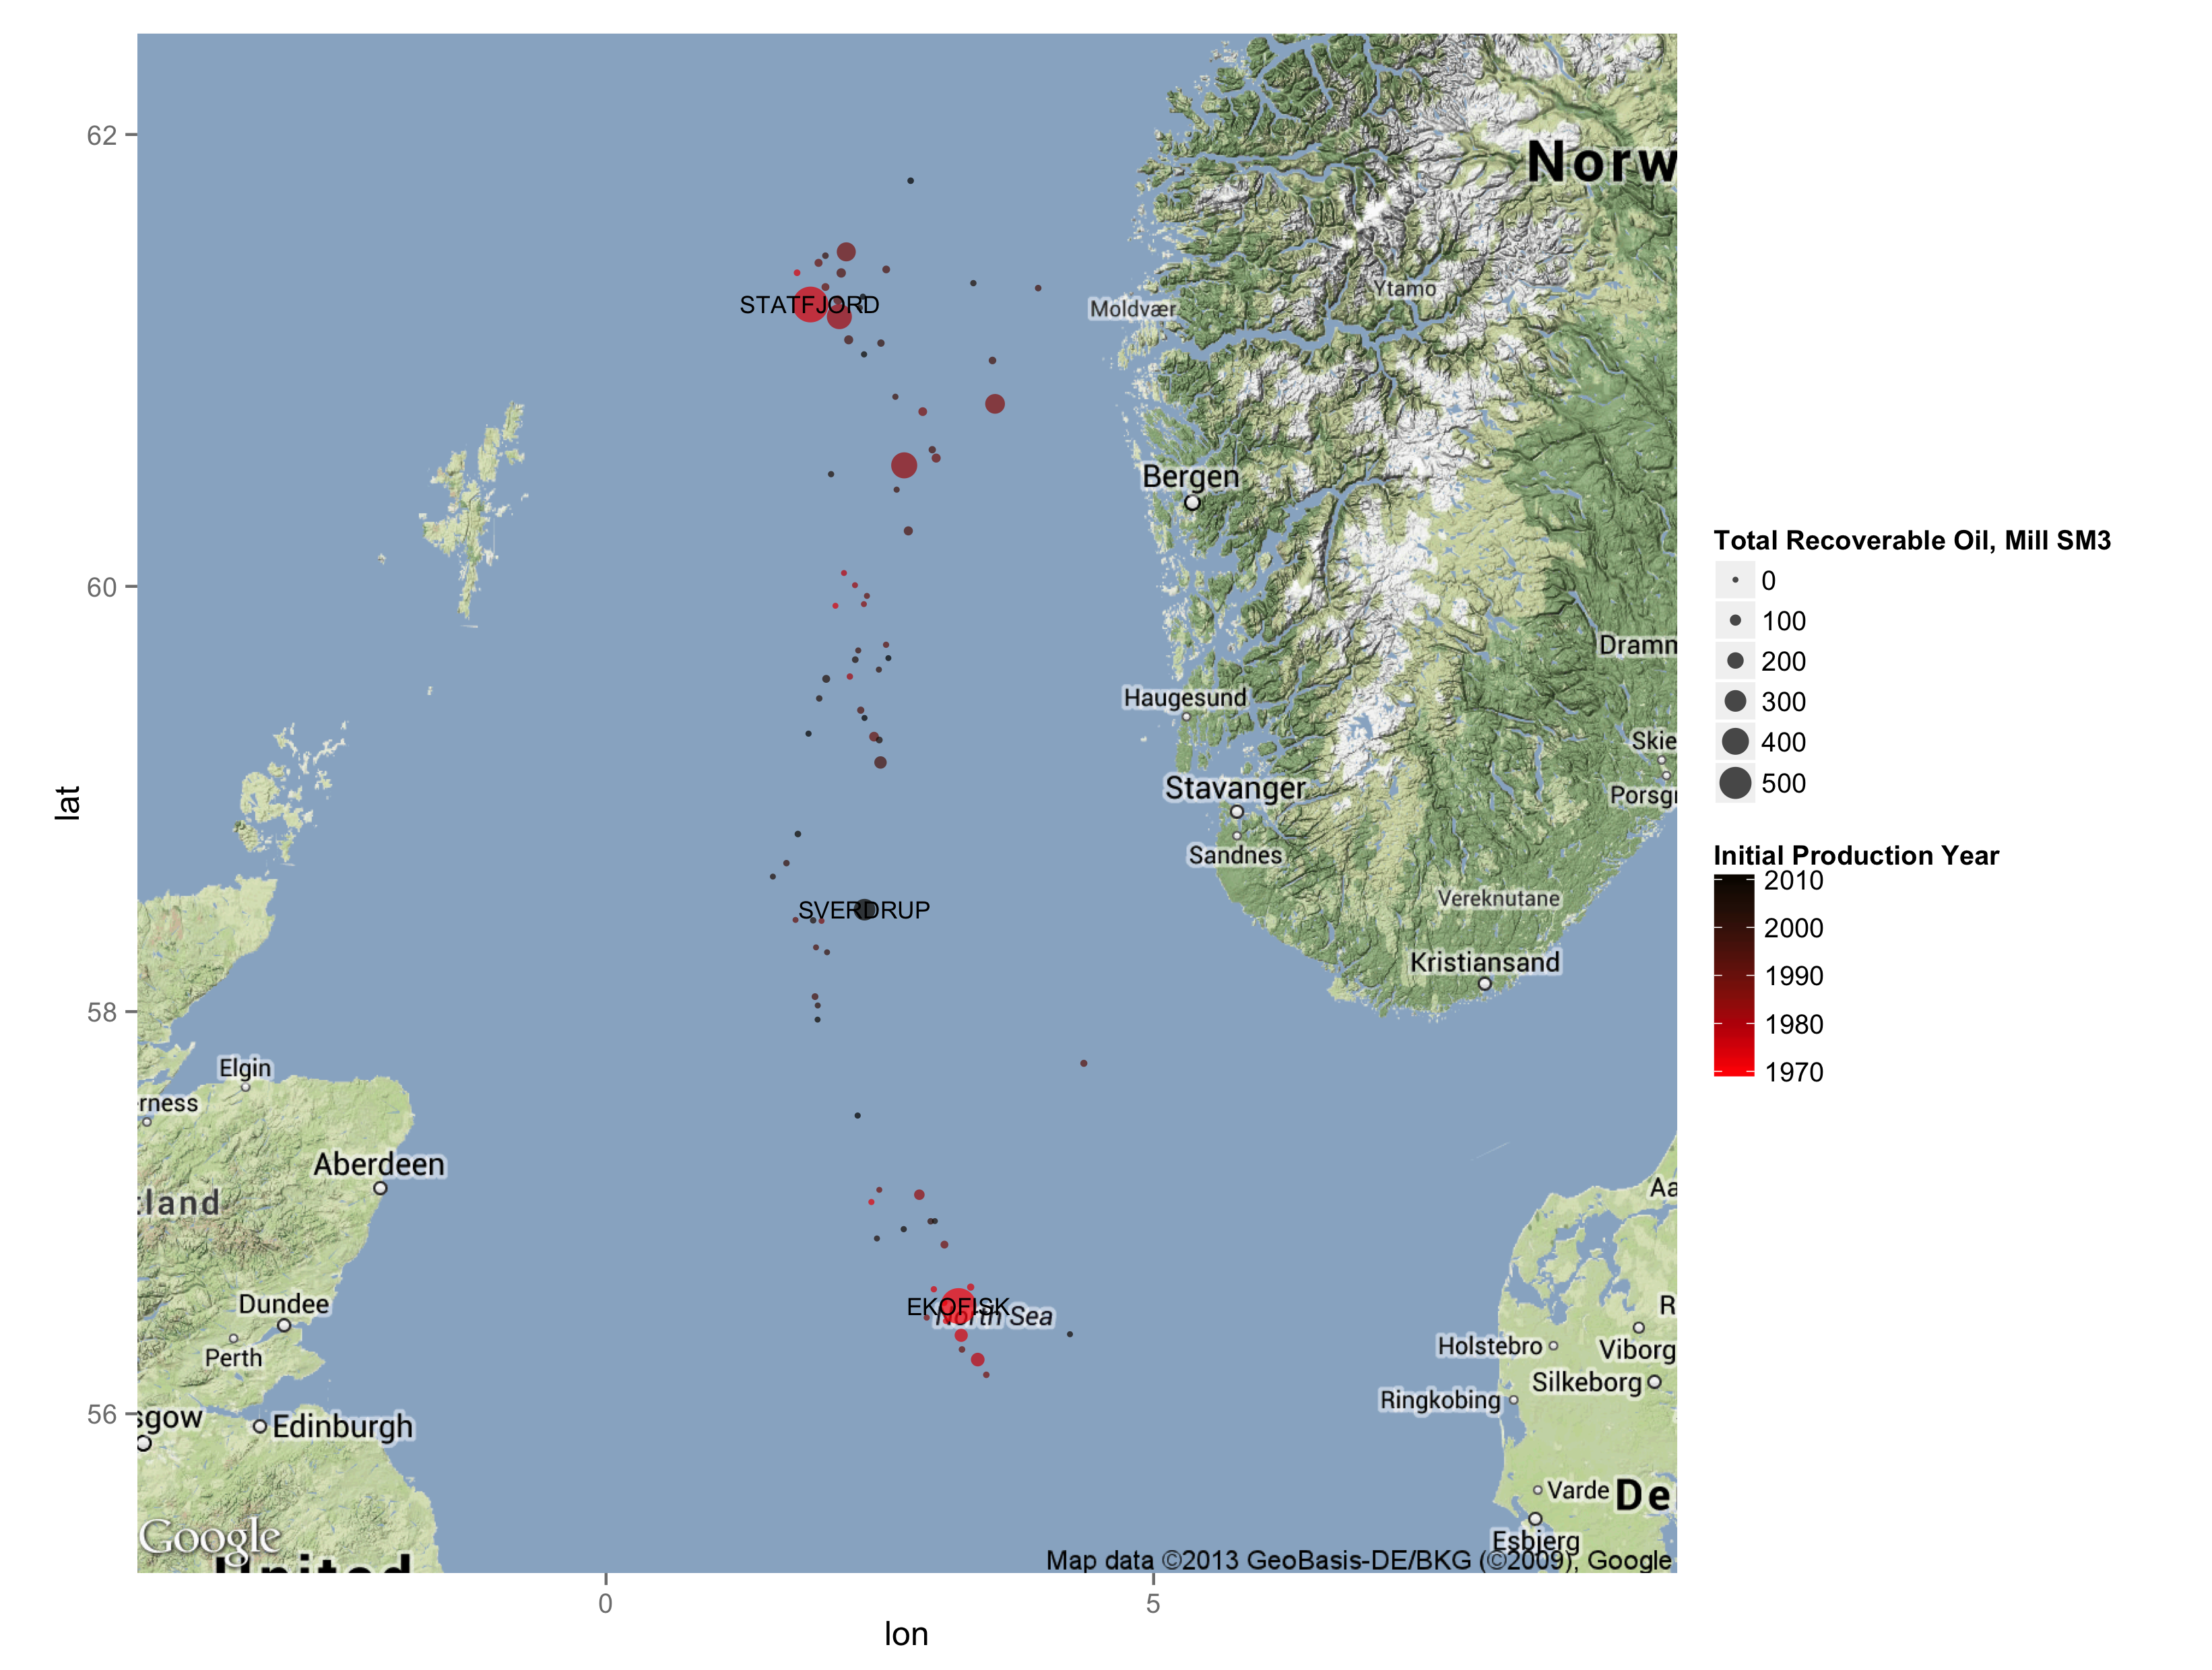
\includegraphics[width=1\textwidth]{north_sea_reserves.png}
\end{figure}

Exploration in the Norwegian sea was opened up for exploration in 1980 and the first commercial field started production in 1981.  While several mid-sized fields have been discovered, the Norwegian Sea has generally dissapointed in terms of oil exploration and most finds have been relatively small (figure 3).  


\begin{figure}
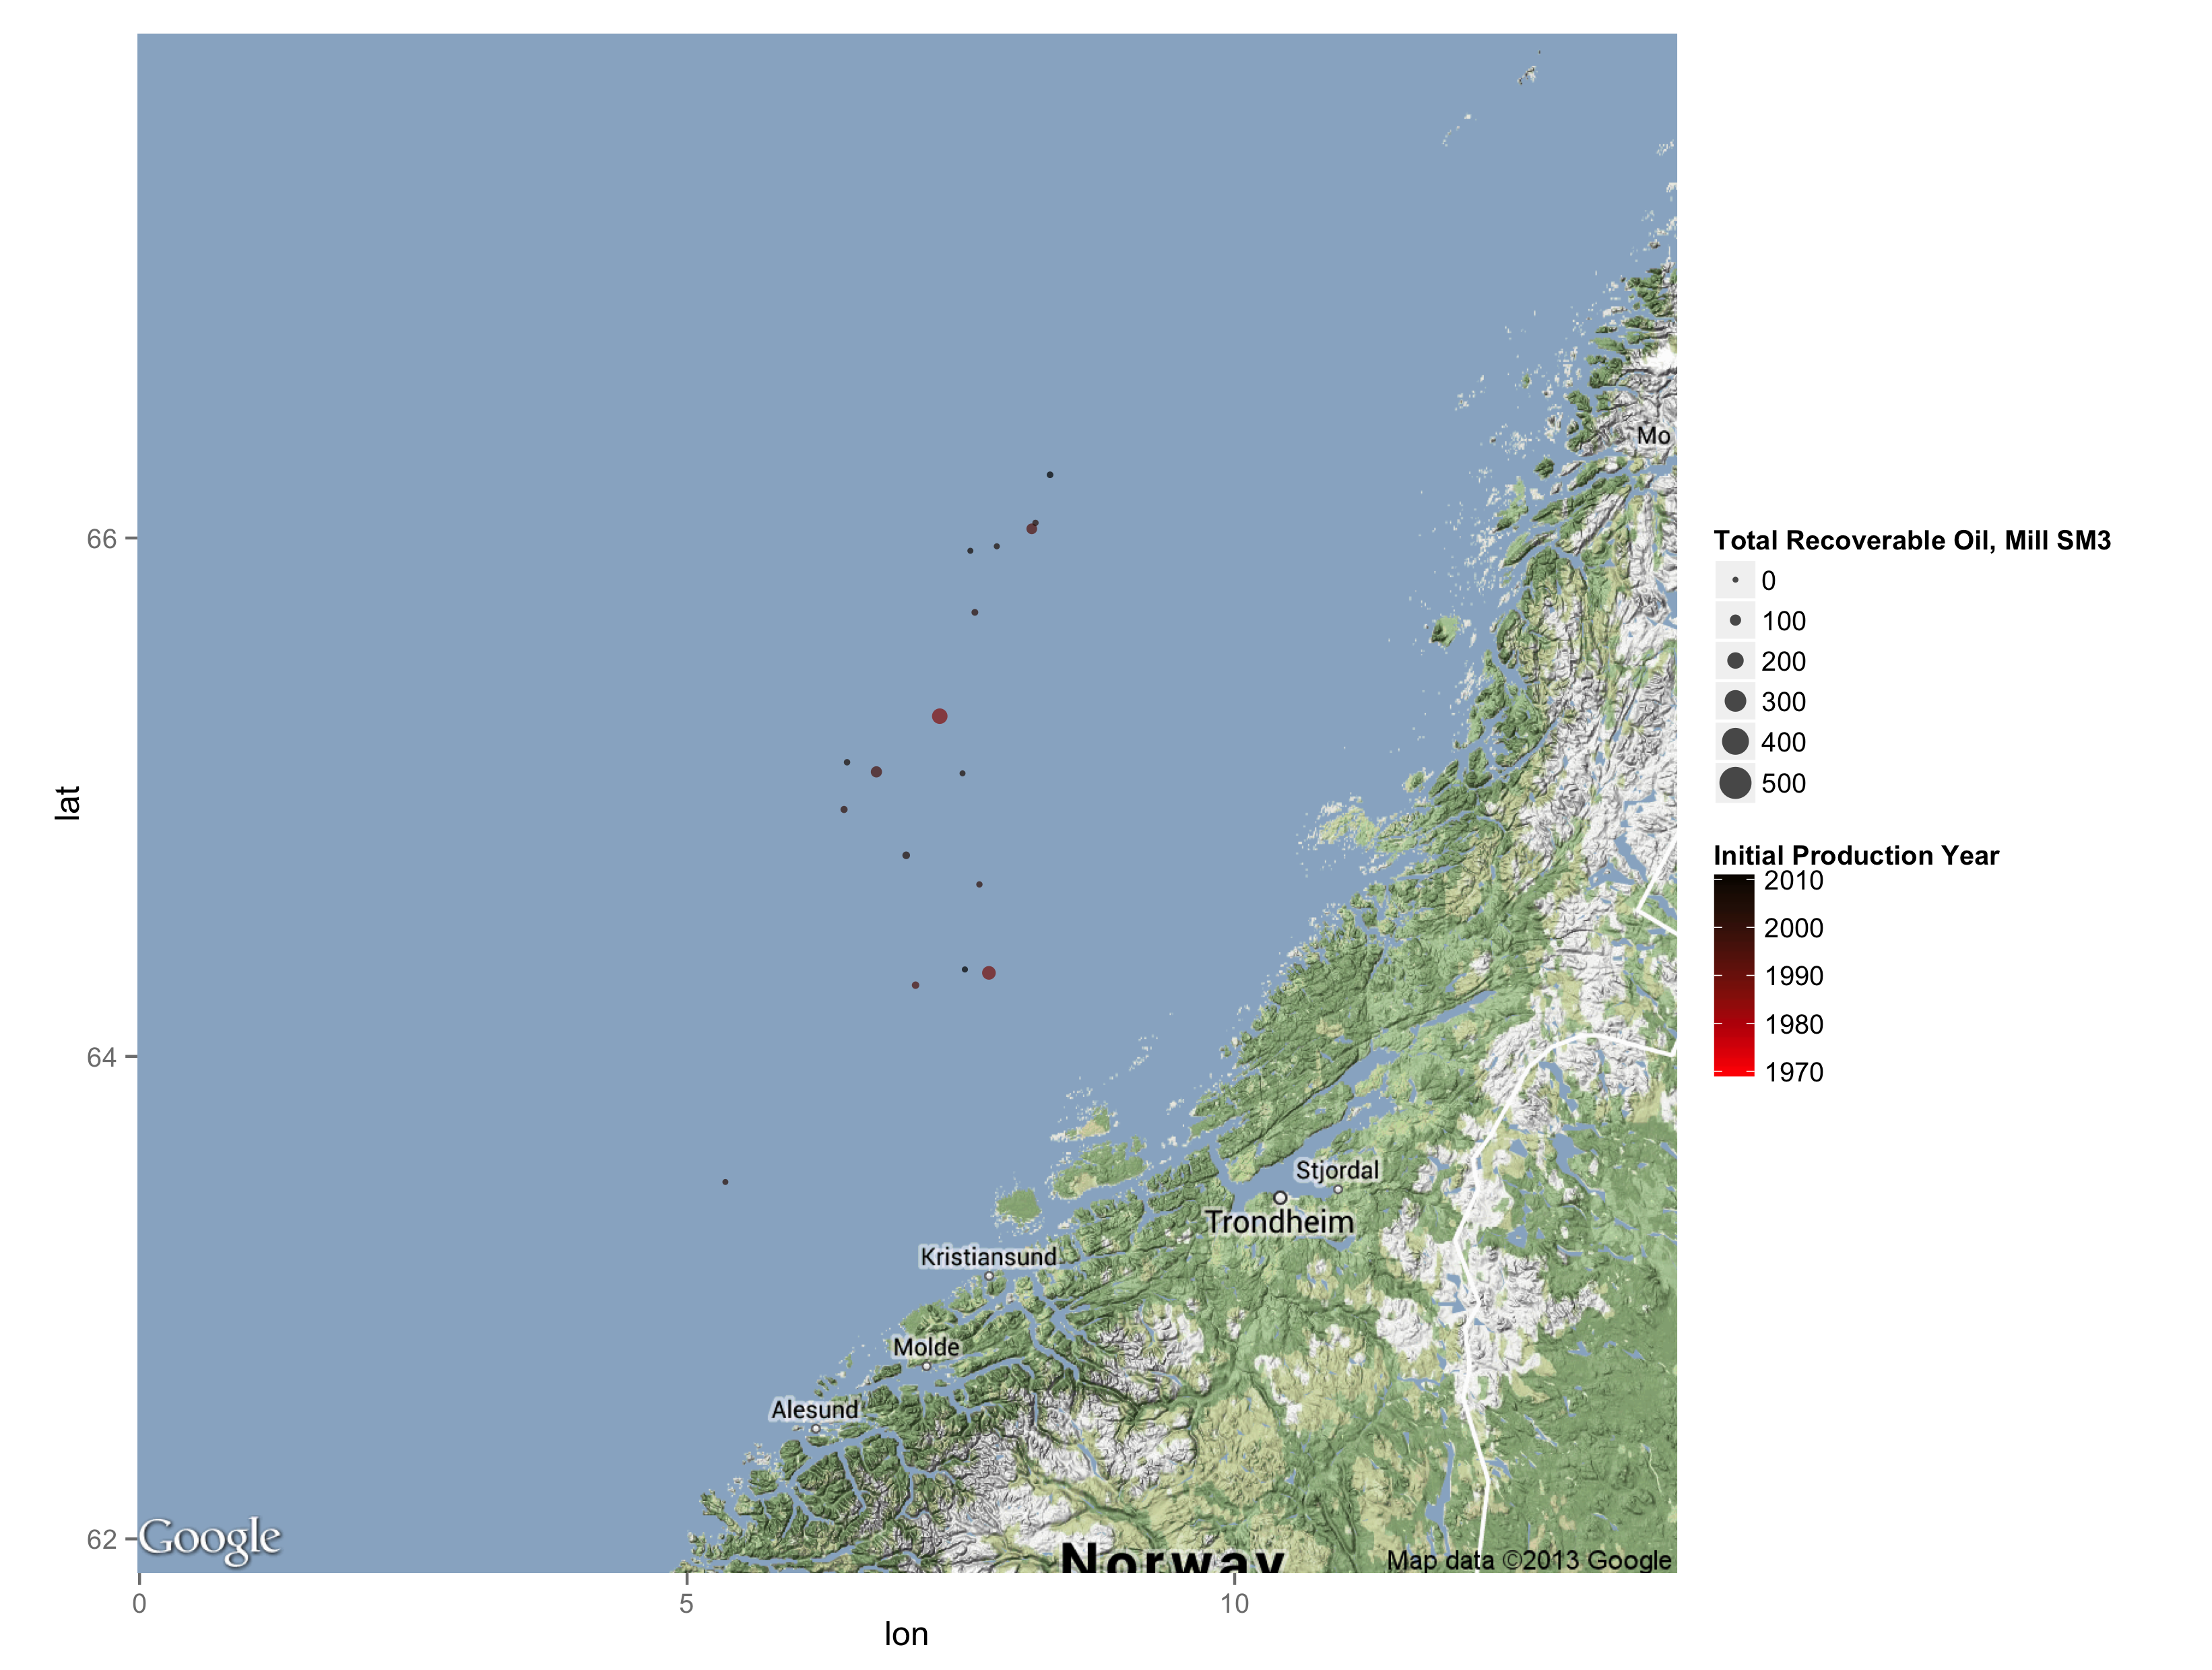
\includegraphics[width=1\textwidth]{norwegian_sea_reserves.png}
\end{figure}

\section{A generalized additive model of oil field production}
	a. Getting a causal interpretation on the coefficient of the oil price variable
		-oil is globally 
	b. comparison to the ideal experiment.  
	To clearify the discussion of causality as well as the limitations of this study I find it useful to describe a hypothetical ideal experiment (as suggested by Gelman and Hill 2007)

\bibliographystyle{abbrv}
\bibliography{main}

\end{document}
This is never printed